Afin d'atteindre les objectifs définis par le cahier des charges du stage, le travail a été réalisé en plusieurs étapes.

\subsubsection{Documentation}
Fund KIS avait déjà repéré les technologies à utiliser pour réaliser la mission du stage. Il s'agit notamment de \href{https://getkong.org}{Kong} \footnote{voir \url{https://getkong.org}}, un \textit{API Gateway} open-source c'est-à-dire un gestionnaire d'API ; \href{https://swagger.io}{Swagger} \footnote{voir \url{https://swagger.io}}, un \textit{framework OAS (OpenAPI Specification)} pour gérer la documentation d'API et \href{https://www.docker.com}{Docker} \footnote{voir \url{https://www.docker.com}}, un gestionnaire de \textit{containers}. Au début du stage nous ne connaissions pas précisément à quoi servait chacun de ces différents outils. Nous nous sommes alors documentés sur chacunes de ces technologies ; c'était la première phase de la documentation. La suite a consité à étudier comment les utiliser pour réaliser notre travail.

\vspace{3mm}

Docker est déjà utilisé par Fund KIS pour le déploiement de ses applications dans des \textit{containers} en production. Un \textit{container} permet d'encapsuler une application en un format qui lui permet de tourner de façon indépendante. On peut le voir comme une machine virtuelle mais il n'est lié à aucun système d'exploitation. Il contient juste les bibliothèques et les paramètres permettant à l'application de tourner toute seule. Cela permet de s'assurer que l'application tournera quel que soit l'endroit où il est déployé puisque c'est un système complètement autonome qui contient tout ce dont il a besoin pour fonctionner.


\vspace{3mm}
Swagger est un \textit{framework} qui permet de suivre une certaine spécification pour gérer la documentation des API. Il permet d'expliquer simplement dans la documentation l'architechture \textit{RESTful} de l'API en détaillant les ressources et les opérations qu'on peut utiliser sur l'API. En utilisant \href{https://github.com/Surnet/swagger-jsdoc}{swagger-jsdoc}, on peut écrire toute la documentation de l'API comme commentaires dans le code source de l'API ; ceci est très intéressant car il permet d'avoir une documentation synchrone avec l'évolution de l'API. Les aspects concernant l'automatisation des documentations des API ont été traités par la deuxième statgiaire avec qui j'ai travaillé.

\vspace{3mm}

Kong est un \textit{API Gateway} et permet de gérer les problématiques de sécurité, d'authentification et de limites d'utilisations des API. On trouvera à la figure 1 suivante un schéma représentant le fonctionne de Kong et des \textit{API Gateway} en général. Il propose une interface \textit{RESTful} et utilise une architecture très modulaire en utilisant des \textit{plugins}. Ainsi on peut le configurer à souhait en utilisant seulement les \textit{plugins} dont on a besoin. On peut même écrire ses propres \textit{plugins} mais il faut pour cela maitriser Lua (langage de programmation).

\begin{figure}[!h]
\centering
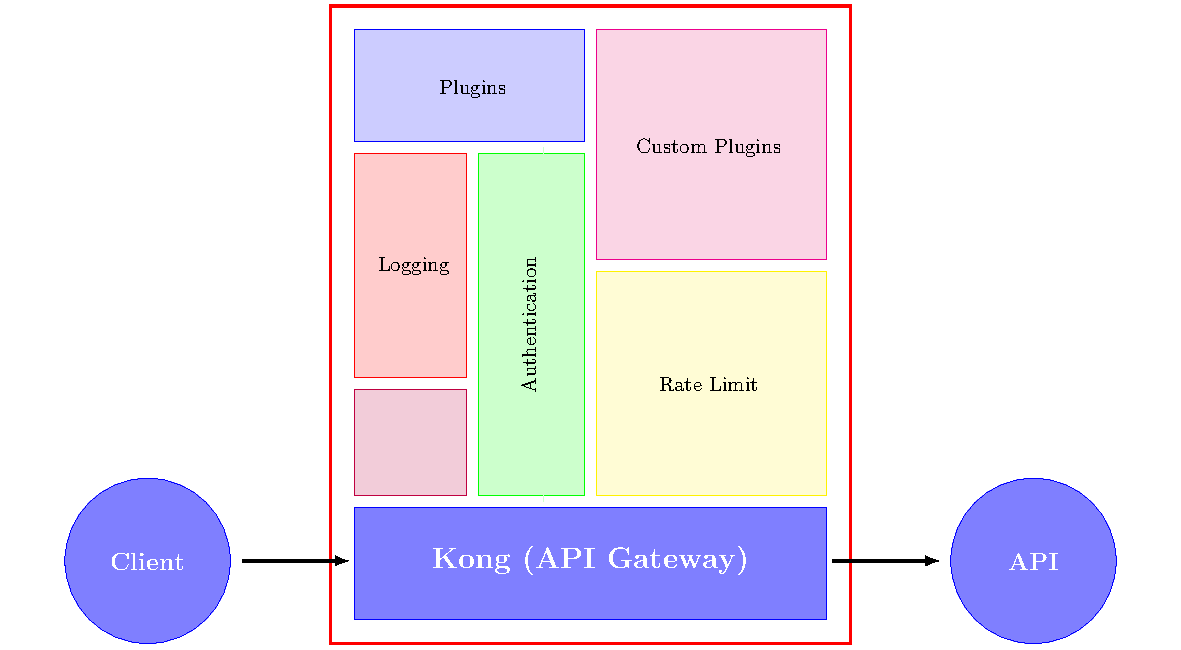
\includegraphics[width=\linewidth]{apigateway}
\caption{Structure d'un \textit{API Gateway}}
\end{figure}

\vspace{3mm}

Cependant, Kong impose une grosse contrainte : il faut absolument une base de données \textit{Cassandra} pour l'utiliser. Mais Fund KIS utilise des bases de données Mongo et SQL. Utiliser Kong comme gestionnaire d'API reviendrait à copier des données des bases données déjà utilisées par l'entreprise dans la bases de données \textit{Cassandra} que Kong va utiliser. Cela est est fastidieux et risque de poser des problèmes d'inconsistance lorsque des données sont mises à jour dans les bases. Même si Kong semblait être une solution adapté à nos problématiques, nous avons dû nous en passer.


\subsubsection{\textit{Rate limiter}}
Le rate limiter

\vspace{3mm}

Middleware qui va avec


\subsubsection{API auto-documentée}
Les navs




% \vspace{5mm}
%
% \begin{figure}[!h]
% \centering
% 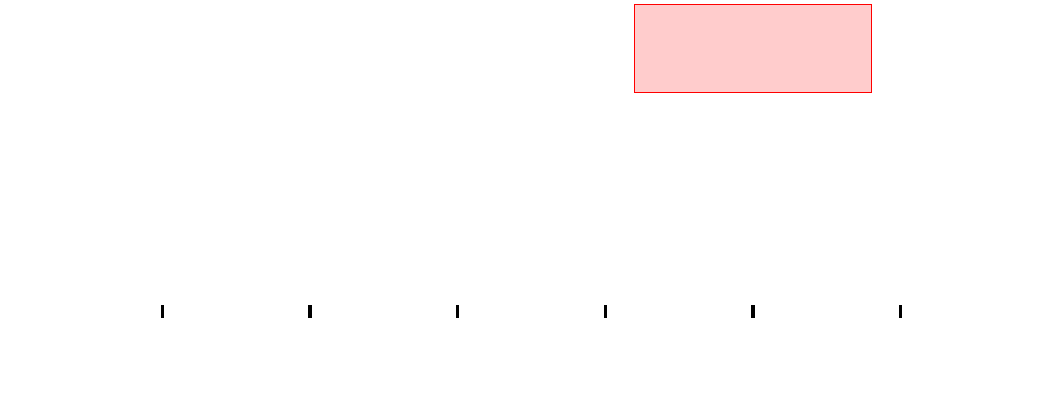
\includegraphics[width=\linewidth]{documentation}
% \caption{Caption}
% \end{figure}
